\begin{frame}
  \frametitle{Algoritmos de Acompanhamento em Tempo Real}
  Existem desde a década de 1980 e ainda atraem bastante pesquisa.\pause\\
  Essa tecnologia tem sido usado em aplicações práticas.\pause
  \begin{itemize}
    \item Antescofo\\
    \item Tonara
  \end{itemize}
\end{frame}

\begin{frame}
  \frametitle{Estratégias utilizadas}
  \begin{itemize}
    \item Inicia-se com uma representação simbólica, como um arquivo MIDI ou MusicXML\\\pause
    \item Converte-o para um arquivo de áudio, usando um software sintetizador\pause
      \begin{itemize}
        \item O problema se reduz a um alinhamento áudio-áudio\\\pause
        \item Sabe-se o tempo de cada evento\\
      \end{itemize}
  \end{itemize}
\end{frame}

\begin{frame}
  \frametitle{Nova estratégia}
  \begin{itemize}
    \item Primeiramente utilizamos uma outra performance da música e a alinhamos com a partitura de forma automatizada\\\pause
    \item Depois, utilizamos essa ``performance anotada'' como nova representação para o processo de rastreamento online\pause
  \end{itemize}

  As motivações são:\pause
  \begin{itemize}
    \item Qualidade das características extraídas\\\pause
  %\note[item]<100>{O arquivo de áudio tem qualidade maior do que uma síntese}
    \item Complexidade perdida na notação musical, que aparece em uma performance\pause
%\note[item]<100>{Como trilos, por exemplo}
  \end{itemize}
  Porém, temos também uma desvantagem:\pause
  \begin{itemize}
    \item A qualidade do processo fica dependente da performance\\
  \end{itemize}
\end{frame}

\begin{frame}[label=figura1]
  \frametitle{Nova estratégia}
  \begin{figure}[!ht]
    \centering
    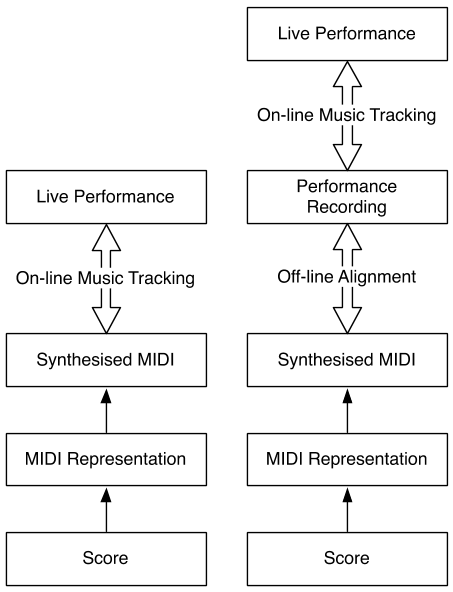
\includegraphics[height=0.7\textheight]{src/img/2-Figure1-1.png}
    \caption*{Rastreamento padrão (esquerda), rastreamento utilizando uma performance como referência (direita)}
  \end{figure}
\end{frame}
